% !TEX TS-program = pdflatex
% !TEX encoding = UTF-8 Unicode

\documentclass[11pt]{article}
\usepackage{ctex}

\usepackage[utf8]{inputenc}
\usepackage{geometry}
\geometry{a4paper}

\usepackage{graphicx}
\usepackage{booktabs}
\usepackage{array}
\usepackage{paralist}
\usepackage{verbatim}
\usepackage{subfig}
\usepackage{fancyhdr}
\usepackage{amsfonts}
\pagestyle{fancy}
\renewcommand{\headrulewidth}{0pt}
\lhead{}\chead{}\rhead{}
\lfoot{}\cfoot{\thepage}\rfoot{}

\usepackage{sectsty}
\allsectionsfont{\sffamily\mdseries\upshape}

\usepackage[nottoc,notlof,notlot]{tocbibind}
\usepackage[titles,subfigure]{tocloft}
\renewcommand{\cftsecfont}{\rmfamily\mdseries\upshape}
\renewcommand{\cftsecpagefont}{\rmfamily\mdseries\upshape}

\title{音乐与数学第20组期中报告}
\author{The Author}

\begin{document}
\maketitle

\part{综述回顾}
音乐的创作是贯穿人类历史中不可或缺的一部分,随着音乐理论的发展与技法的成熟,人们也在不断追寻新的创作理论。在过去的20世纪中,随着数学的发展,特别是随机过程论的建立,使得用\textbf{随机数}来创作音乐成为可能。我们首先回顾这方面已有的工作。
\section{音乐创作实验}
以 \cite{Brooks:1992:EMC:167765.167774} 的工作为例:
\subsection{旧有工作的困难点}
从样本中获取足够的信息,随后对新元素与已经存在的元素进行演绎,不仅取决于分析的复杂性,还取决于所分析的样本的特征。
试想一项工作仅分析少数曲调并且将分析的结果运用于演绎产生新曲调的随机过程。
通常会出现三个困难。
\begin{figure}[hptb]
	\centering
	\label{fig:1.1.1}
	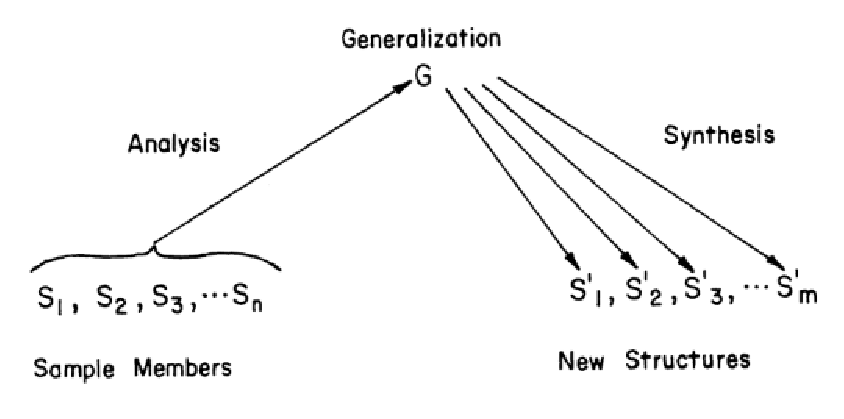
\includegraphics[width=\textwidth]{pic/1.1.1.eps}
	\caption{Figure 1.1.1}
\end{figure}	
如图 \ref{fig:1.1.1} 所示,这个图表显示了将 $S1, \dots, Sn$ 作为样本的分析过程,他们属于某种相同的结构,将其标记为 $G$ 。
从 $G$ 中演绎出来新的结构,标记为 $S'$ ,我们希望它与之前的样本具有相同的结构。
\begin{itemize}
\item 第一个困难点在于太过简单的分析会使得一般化的 $G$ 的结构过于松散,而导致演绎出来的 $S'$ 与之前的样本不属于同一结构。
\item 第二个困难点在于样本量可能太小以至于不管分析多复杂都无法较好地演绎出一个一般化的 $G$ 。
\item 第三个困难点在于当构建一般化的 $G$ 时,样本成员可能十分相像,这可能导致在创建新的结构 $S'$ 时,无法创造出新的与样本 $S$ 结构不同而又属于同一类别的结构。
\end{itemize} 

\subsection{随机过程的方法}
以如下结构 \ref{fig:1.1.2} 为例
\begin{figure}[hptb]
	\centering
	\label{fig:1.1.2}
	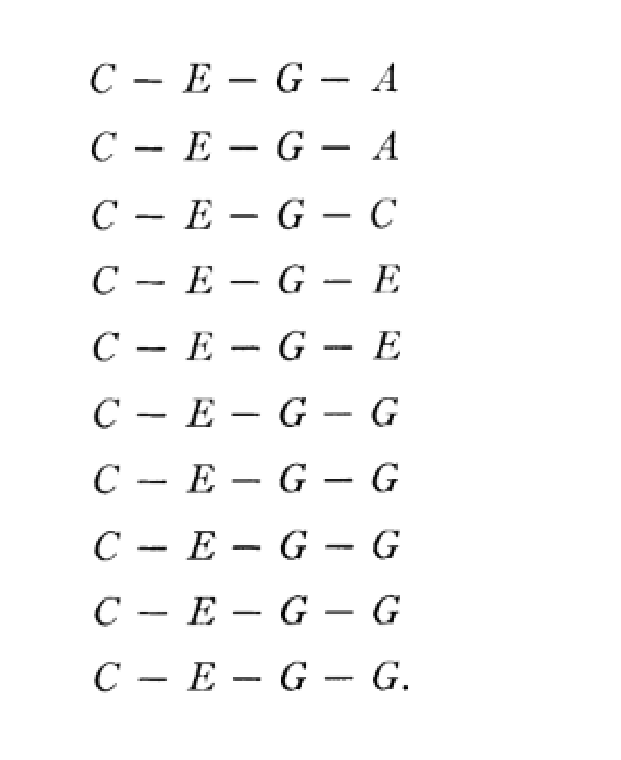
\includegraphics[width=0.5\textwidth]{pic/1.1.2.eps}
	\caption{Figure 1.1.2}
\end{figure}	
我们可以得到,在 C-E-G 后出现 A, C, E, G 的概率分别为
$$ P(A) = 2/10 = 0.2 $$
$$ P(C) = 1/10 = 0.1 $$
$$ P(E) = 2/10 = 0.2 $$
$$ P(G) = 5/10 = 0.5 $$
于是可以将 $[0, 1]$ 划分相应的区间
$$ A \quad 0 \le x < 0.2 $$
$$ C \quad 0.2 \le x < 0.3 $$
$$ E \quad 0.3 \le x < 0.5 $$
$$ G \quad 0.5 \le x < 1.0 $$
那么取值随机的 $x$ 在 $0$ 到 $1$ 取值,当落在 $[0, 0.2)$ 时取 $x$ 为A,其他区间取值与之类似。
\begin{figure}[hptb]
	\centering
	\label{fig:1.1.3}
	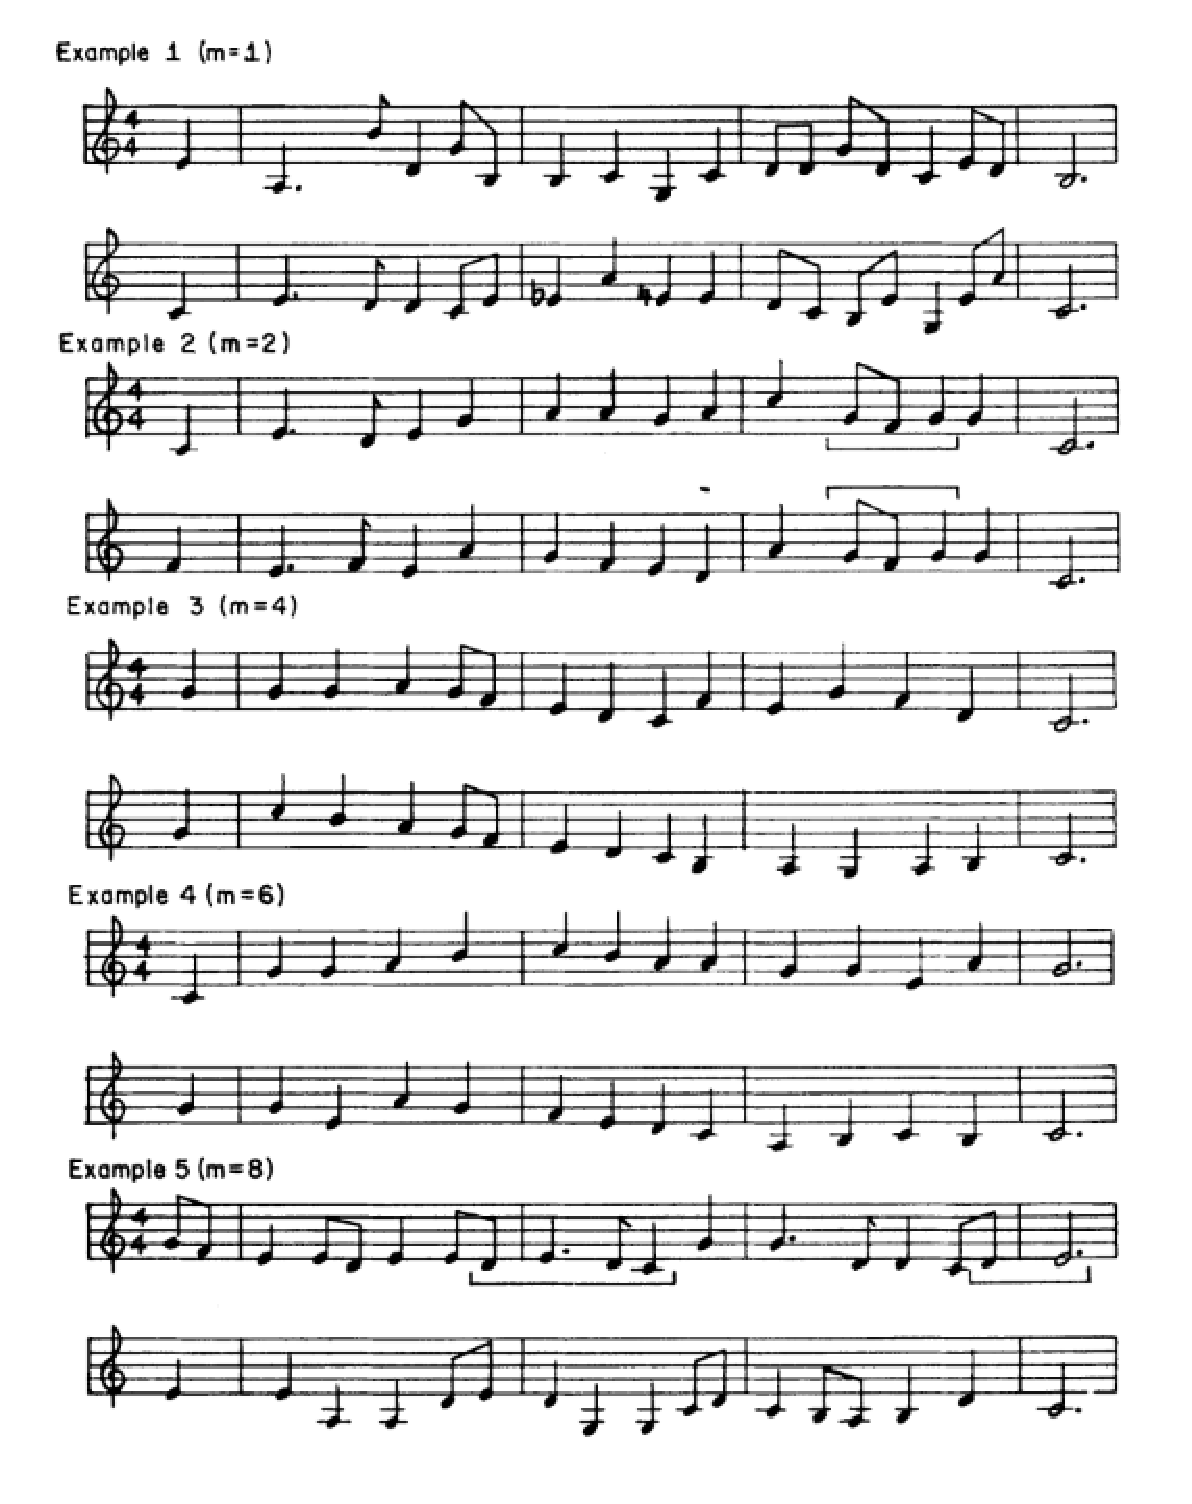
\includegraphics[width=\textwidth]{pic/1.1.3.eps}
	\caption{Figure 1.1.3}
\end{figure}
图 \ref{fig:1.1.3} 为马尔科夫链 $m=1,2,4,6,8$ 时的一个试验结果。

\section{连续音乐领域}
这里我们着眼于 \cite{10.2307/24955701} 的工作。
\subsection{相关背景}
过去的作曲家如果想要得到在纯正的白噪音和布朗噪音之间的作品,他们将会把这种相关关系扩展到三个或者四个音符之间。但是即使由前四个音符决定第五个音符,每五个音符之间还是随机的,因此,现阶段几乎所有的随机音乐都是这样——在小范围内听起来是有艺术性的,但是当你放眼于整段音乐作品的时候,它就是随机的而且并不悦耳。

Voss 则创作了一种严格介于白噪音和布朗噪音之间的噪音,也就是 $1/f$ 噪音,这种噪音的音符在任意范围内都是适当相关的,也被普遍认为比白噪音和布朗噪音更加悦耳。

在电子学领域 $1/f$ 噪音很常见但是却很少有人真正理解。Mandelbrot 也首先意识到,不仅是在物理学,在自然界中 $1/f$ 噪音也是很常见的。此后有很多数学家,通过各种方法得到这种适度相关的曲线。但自然界中的事物没有人造曲线那么规则,他们的自相似性往往需要用统计学数据的协助。而且无论是截然姐还是人工制作,它的自相似性都是有一定的范围的,当放大到足够小的范围的时候,这种相似性就会被打破。

\subsection{$1/f$ 音乐的起源}
早在古希腊时,柏拉图和亚里士多德就认为包括音乐在内的艺术都是在 \textbf{模仿}(imitate)自然。但是我们很难说清音乐具体在模仿什么,特别是纯音乐(absolute music),它除了自己并没有代表其他东西。那么音乐带给我们的愉悦从何而来?它是否在模仿,如果是的话是在模仿什么?

Richard F. Voss的研究表明,好的音乐似乎反映了世界的微妙的统计性质。而关键的概念是谱线密度(spectral density of a fluctuating quantity)以及其自相关(autocorrelation)的性质。

\subsection{白噪声,布朗噪声与 $1/f$ 噪声}
如果一段声音,在加速或放慢播放后,只需调整音量即可使其听着和原速一样,则称为 \textbf{缩放噪声}(scaling noises)。最简单的缩放噪声是\textbf{白噪声}(white noise),两个相邻的音符之间没有任何关联,时值和音高均随机。其次是\textbf{布朗噪声}(Brownian noise),与布朗运动类似。例如,我们可以按顺序一个一个产生音符,音符在钢琴的黑白键范围内,并规定新产生的音符比其之前的音符,有40\%的概率下降一个音级,60\%的概率上升一个音级,这样产生的便是布朗噪声。可以看出这是通过一阶的马尔科夫矩阵产生音乐,也可以用更高阶的马尔科夫矩阵。Voss曾用巴赫的音乐取样,并用3、4阶的马尔科夫矩阵产生音乐,得到的音乐在短范围内与巴赫相似,而大范围内还是杂乱的。

白噪声和布朗噪声是两个极端,白噪声是完全不相关的声音,而布朗噪声是完全相关的声音。如果用谱线密度来考虑这两种噪声,白噪声的谱线密度是与$f$的$0$次方成反比,而布朗噪声是与$f$的$2$次方成反比。而谱线密度介于它们之间的与$f$的$1$次方成反比的噪声,称之为\textbf{flicker noise}或\textbf{$1/f$噪声}。而$1/f$噪声既不完全不相关,也不完全相关。

\begin{figure}[hptb]
	\centering
	\label{fig:1.2.1}
	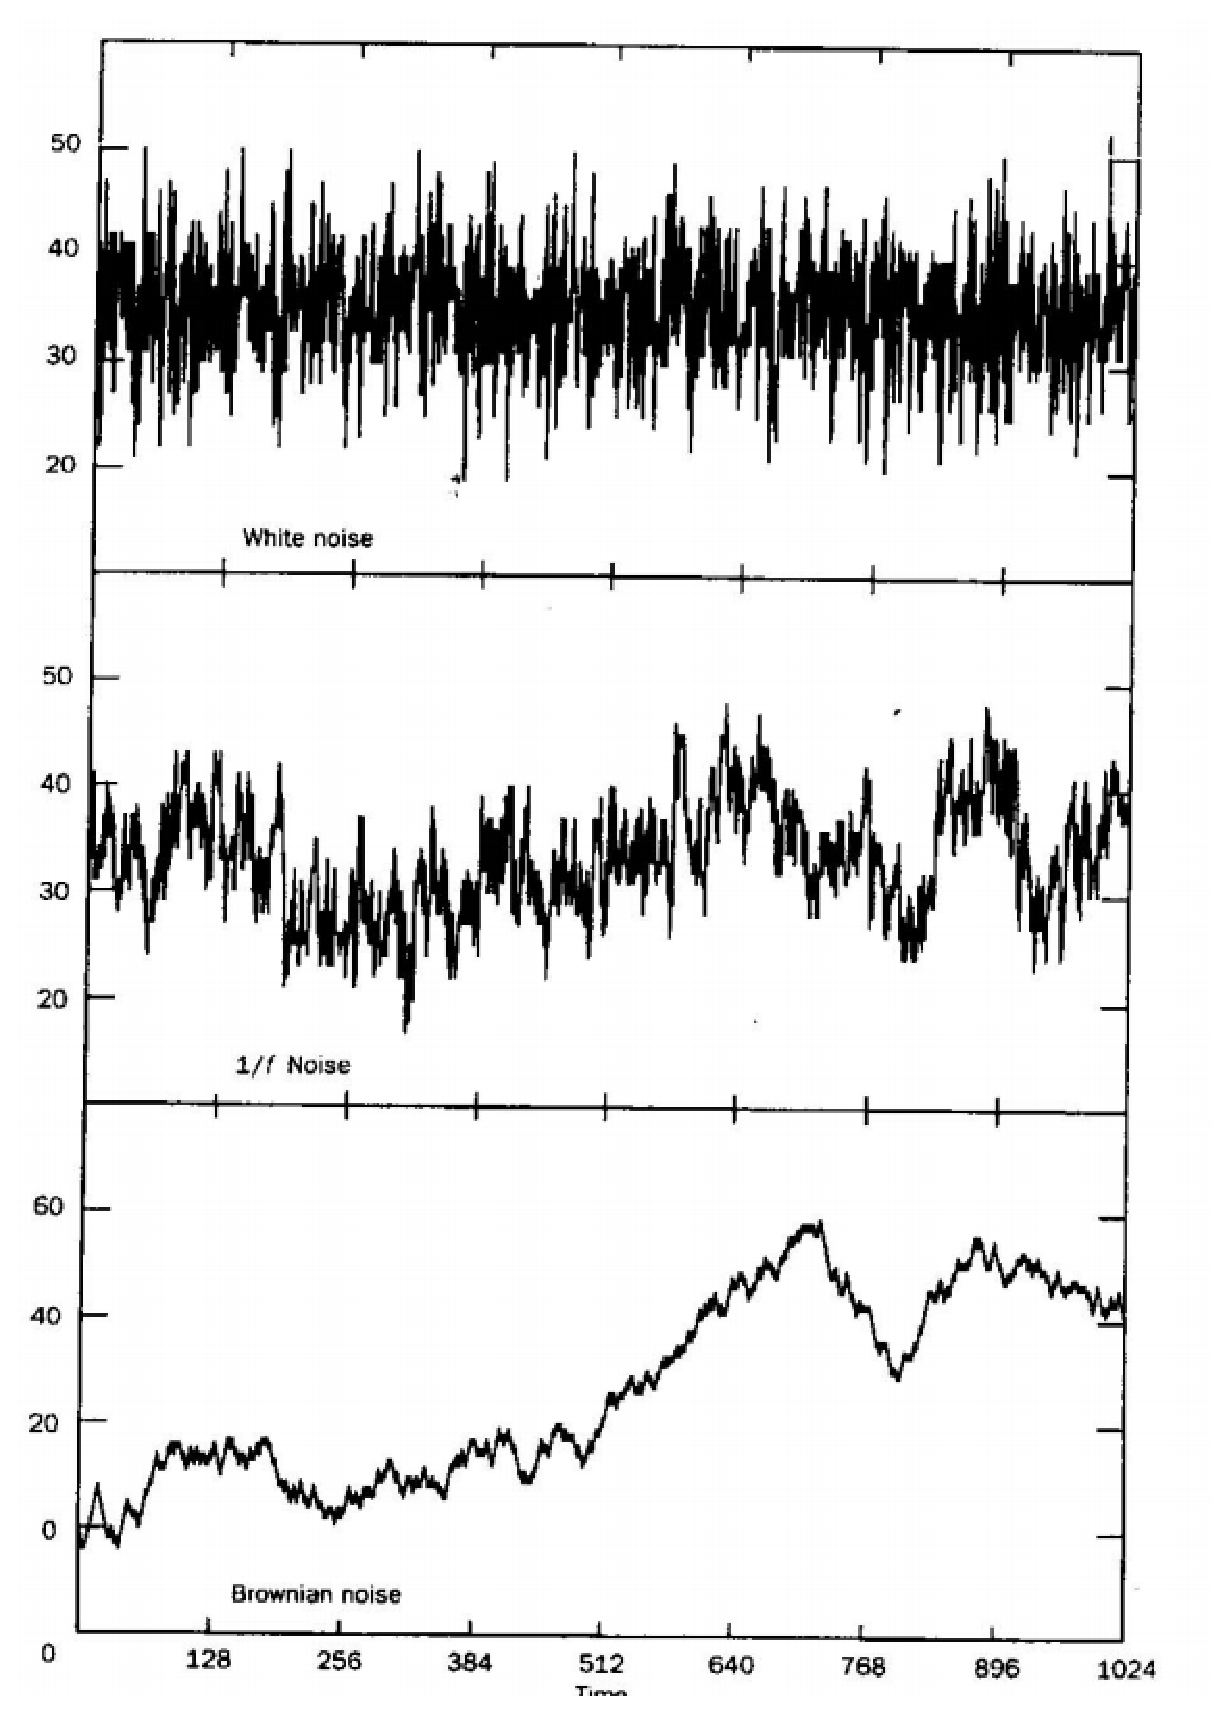
\includegraphics[width=\textwidth]{pic/1.2.1.eps}
	\caption{Figure 1.2.1}
\end{figure}

\subsection{世界中的 $1/f$ 噪声}
静态世界中,存在大量与布朗噪声相似的分形结构,即存在大量与$f$的$2$次方成反比的谱线密度的波动量。例如,用布朗噪声的音高映射成高度,产生的图像与大自然中的山类似。

\begin{figure}[hptb]
	\centering
	\label{fig:1.2.2}
	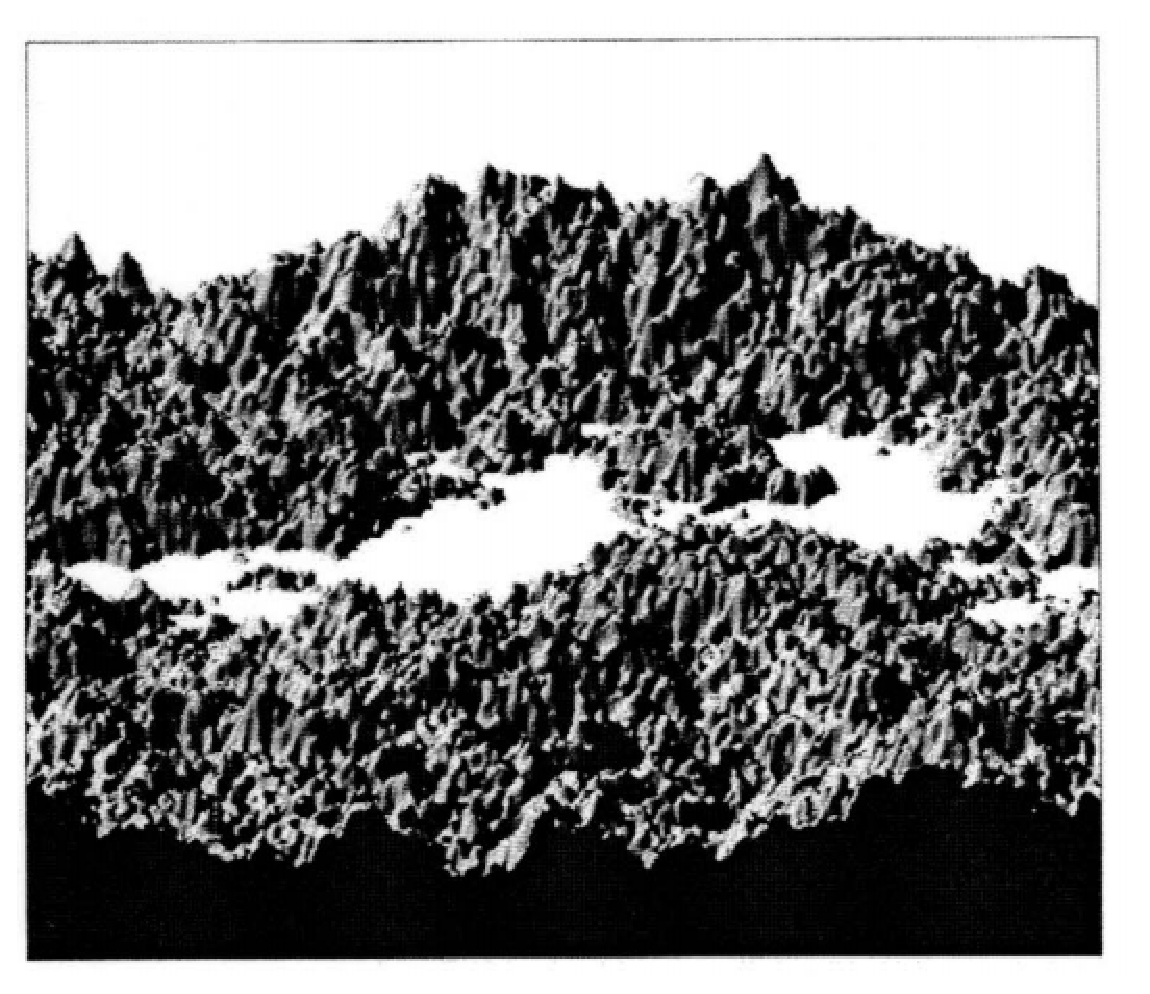
\includegraphics[width=0.5\textwidth]{pic/1.2.2.eps}
	\caption{A modified Brownian landscape generated by a computer program}
\end{figure}

然而,在动态的世界中,$1/f$的谱线密度无处不在。T. Musha曾用激光去扫描周围大片的地形,以激光能走的距离作为波动量,产生的是布朗噪声的谱线。但当他在不同时间扫描两次,并将两个谱线作差,得到的是$1/f$谱线。也就是说世界的变化(我们所经历的内容变化)聚集在$1/f$附近。而音乐就是在模仿我们所经历的内容变化的$1/f$性质。

\subsection{生成}
下面,我们利用骰子产生三种噪声。
\begin{itemize}
\item 白噪声:扔三个骰子,得到的数字和(3-18)分别对应16个音符。不断重复。
\item 布朗噪声:扔一个骰子,奇数音级+1,偶数音级-1.
\item $1/f$噪声:三个骰子,分别是红、蓝、绿色的。他们投出的数字的总和(3-18)分别对应16个音符。
\end{itemize}
现在我们要产生一段8个音符的片段。将0~7对应成二进制的000~111,每一位对应一个骰子(如图\ref{fig:1.2.3}所示)

\begin{figure}[hptb]
	\centering
	\label{fig:1.2.3}
	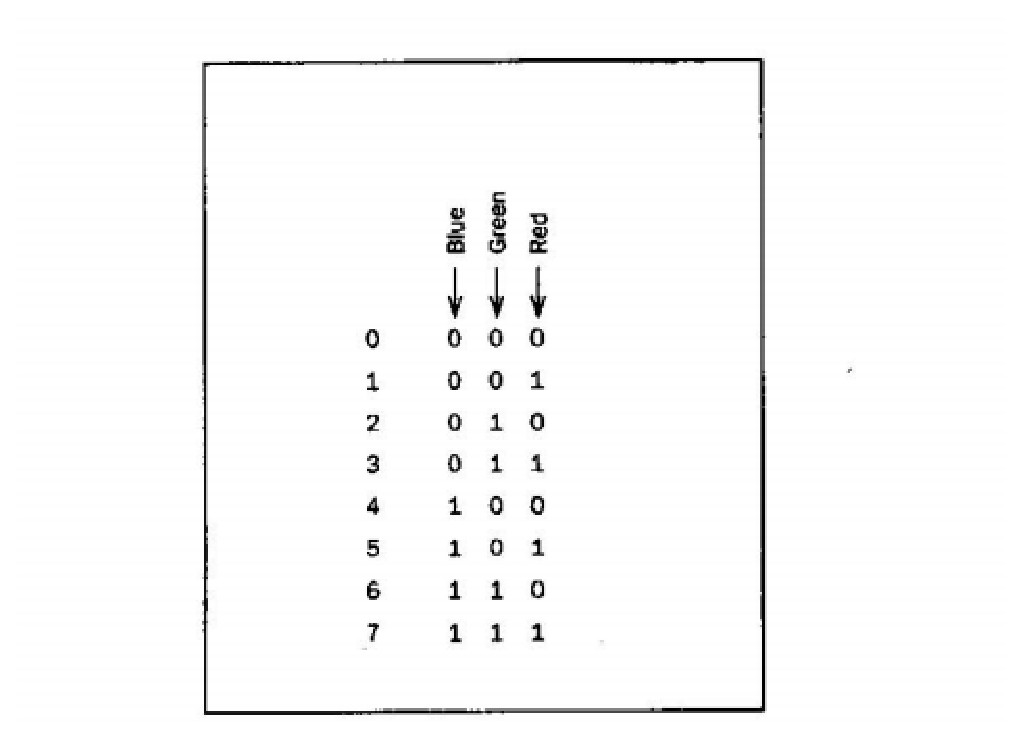
\includegraphics[width=0.4\textwidth]{pic/1.2.3.eps}
	\caption{Binary chart for Voss's $1/f$ dice algorithm}
\end{figure}

我们先扔出三个骰子,得到数字和产生对应的第一个音符。在产生第二个音符时,由于000到001只有红色对应的位数字变了,只投红骰子,蓝绿骰子的数字不变,由此得到的数字和产生对应的第二个音符。在产生第三个音符时,001-010,红色和绿色对应的位数字都变了,所以蓝色数字不变,投红和绿骰子,由此得到的数字和产生对应的第三个音符。以此类推。

可以看出,对应位数高的骰子投的频率低,位数低的投的频率高,在多次数的平均过后,产生的就是$1/f$噪声了。当我们可以利用更多的骰子产生更长、音域更广的音乐片段。

Voss利用这样的算法产生了一些音乐片段,并做实验给一些人听,得到的反馈是:
白噪声过于随机,布朗噪声过于相关,而$1/f$刚刚好。他还将$1/f$应用于5音阶,产生的片段接近东方音乐。

\subsection{性质}
$1/f$音乐具有自相似性,在小范围内,音符与音符之间是$1/f$;在大范围内,小段与小段之间也是$1/f$。$1/f$音乐似乎\emph{有记忆},每段音乐与过去总是有某种程度的关联。$1/f$音乐是秩序与意外的结合,有意外的前提是有秩序,而毫无意外则显得无趣。

$1/f$音乐在经过倒放、音高反转(以五线谱的某条线将音符上下对称)变换下依然是$1/f$音乐。


\part{基于马尔科夫链的随机音乐}
\section{一般理论基础}
考虑音符序列 $S=\{X_1, X_2, \dots, X_n\}$ ,其中 $X_i$ 是单个音符单位。我们希望 $S$ 服从给定序列 $S_0 = (Y_1, \dots, Y_m)$ 的转移概率。这是通过以下两个步骤实现的:
\begin{enumerate}
\item 根据 $S_0$ 计算转移概率张量 $P$ 。一般地,考虑 $k \ge 1$ 阶的转移概率矩阵 $P$ 的第 $(i_1, i_2, \dots, i_k)$ 项:
$$
P(i_1, i_2, \dots, i_k) = \frac{\#\{l|Y_l=i_1, Y_{l+1}=i_2, \dots, Y_{l+k-1}=i_k\}}{m-k+1}
$$
\item 根据张量 $P$ 生成序列 $S$ 。考虑给定初始状态 $X_1, \dots, X_{k-1}$ ,那么 $X_q(q \ge k)$ 由 $X_{q-k+1}, \dots, X_{q-1}$ 决定,其条件概率为
$$
\mathbb{P}(X_q=j|X_{q-k+1}=i_1, \dots, X_{q-1}=i_{k-1}) = \frac{P(i_1, \dots, i_{k-1}, j)}{\sum_l P(i_1, \dots, i_{k-1}, l)}
$$
\end{enumerate}
接下来我们讨论关于 $X_i$ 的细节。程序实现请参见 \begin{verbatim}https://github.com/owen8877/markov-midi\end{verbatim} 。
\subsection{单声部仅音高情形}
我们姑且认为 $X_i$ 是取值于 MIDI 音符标准集 \{A0, \dots, C8\} 中的随机变量。
\subsection{单声部考虑音高与时值情形}
我们姑且认为 $X_i=(p_i, d_i)$ 是由音高 $p_i$ 与时值 $d_i$ 组成的二元对,$p_i$ 取值于 MIDI 音符标准集 \{A0, \dots, C8\} 中的随机变量, $d_i$ 取值于 $\mathbb{R}$ 或 $\{\dots, 2^{-2}, 2^{-1}, 2^{0}, 2^{1}, 2^{2}, \dots\}$。
\subsection{耦合多声部仅音高情形}
由于多声部的每个声部并不一定遵循相同的节奏规律,因此我们将音符序列切割为它们的最小时值单位,此时 $X_i=(p_{1i}, \dots, p_{si})$ ,这里 $s$ 是声部的数目。
\subsection{独立多声部仅音高情形}
与上述情况不同的是,我们独立统计每个声部的转移概率矩阵并进行随机模拟。

\section{数值实验}
我们选择了广泛的音乐序列来源,分别有
\begin{enumerate}
\item \textbf{cuphead.mid} 横版射击游戏 Cuphead 中的背景音乐 \emph{Inkwell Isle One}
\item \textbf{K465.mid} 莫扎特第 19 首弦乐四重奏 \emph{不和谐音} 第一乐章的引子部分
\item \textbf{Mahler.mid} 马勒第五交响曲第四乐章
\item \textbf{RV156.mid} 维瓦尔第 g 小调弦乐协奏曲第一乐章
\end{enumerate}
对于这些乐曲,我们分别生成了相应的随机乐曲,以下是一些参考输出:
\begin{enumerate}
\item \textbf{K465-compound-deg4-Violin-Violin-Viola-Cello} 4 阶四声部,基于 K465 而作。
\begin{figure}[hptb]
	\centering
	\label{fig:K465-compound-deg4-Violin-Violin-Viola-Cello}
	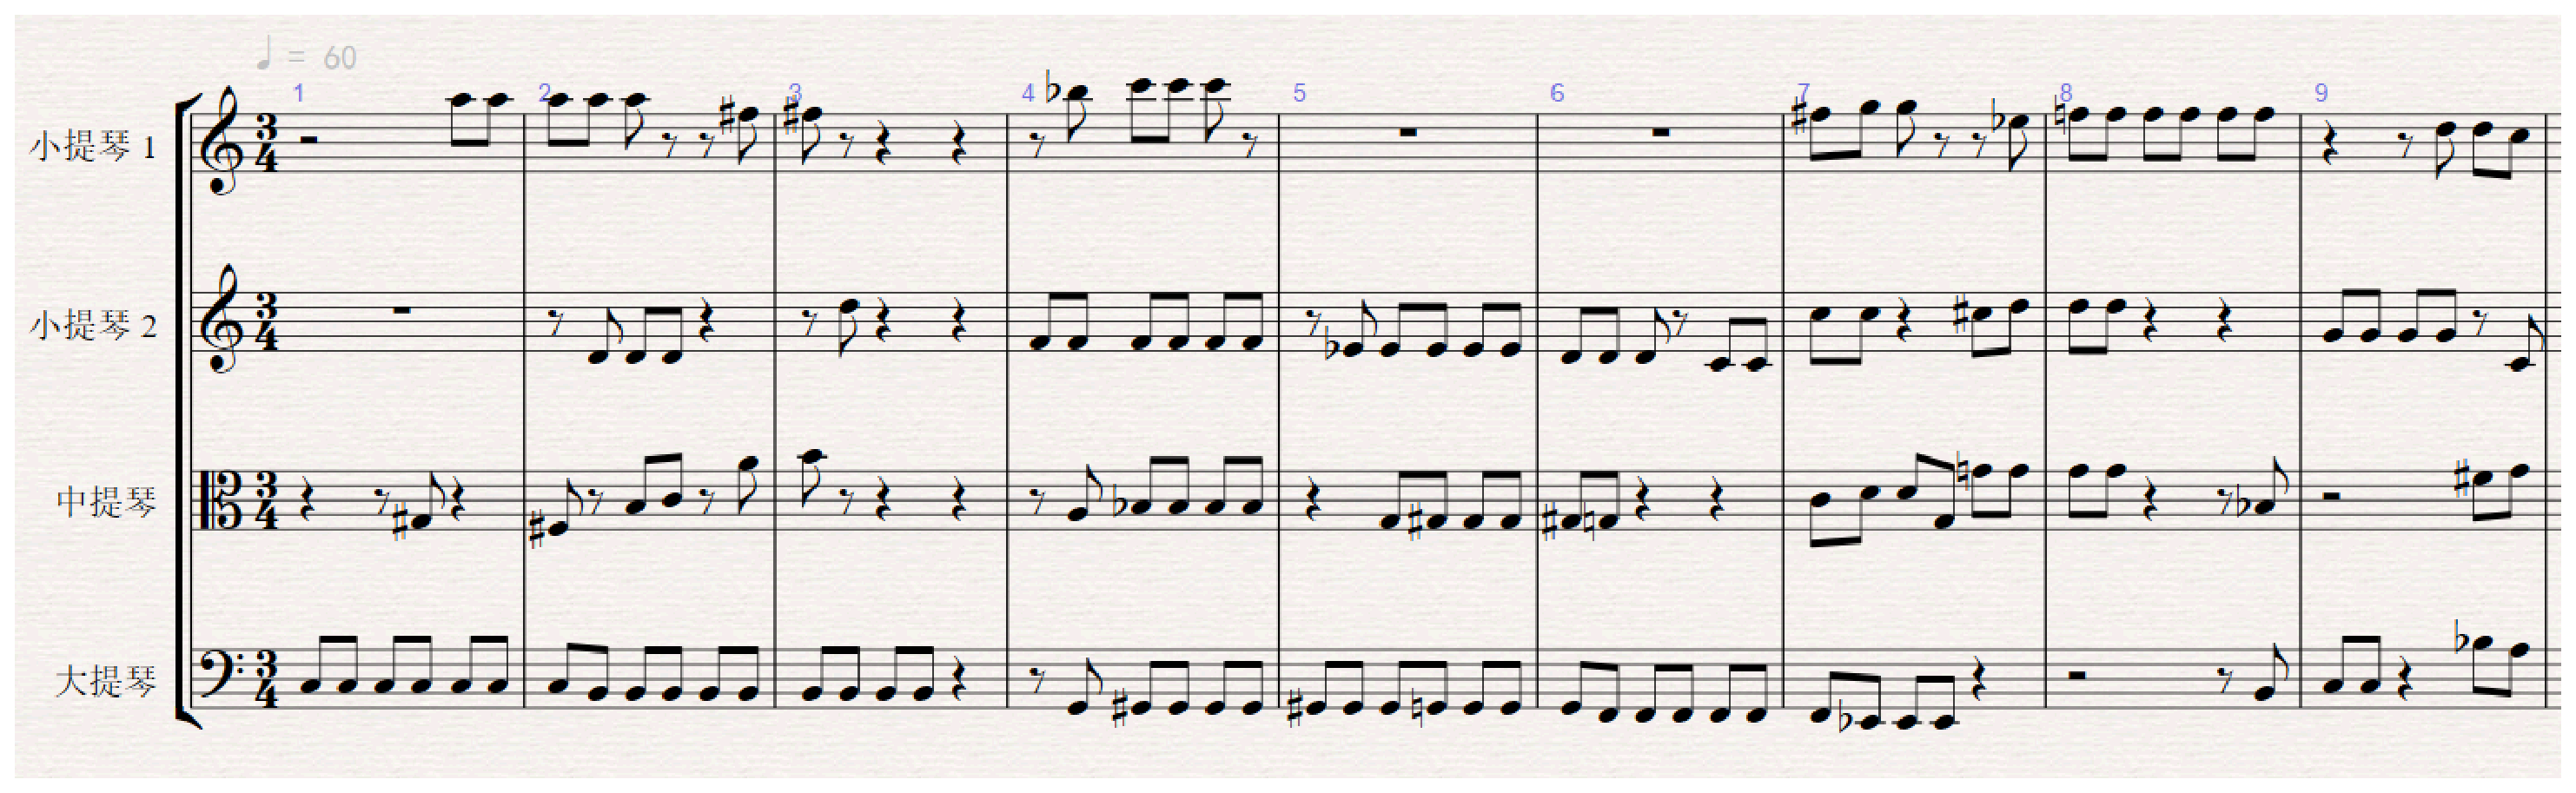
\includegraphics[width=\textwidth]{pic/K465-compound-deg4-Violin-Violin-Viola-Cello.eps}
	\caption{K465-compound-deg4-Violin-Violin-Viola-Cello}
\end{figure}
\end{enumerate}

\bibliographystyle{apalike}
\bibliography{ref}

\end{document}
